% !TeX program = XeLaTeX
% author: buwailee@nmhs
\documentclass[9pt,twoside,openany,svgnames,x11names]{extbook}
\usepackage[b5paper, top=10mm, text={144mm, 208mm}, includehead, includefoot, hmarginratio=1:1, heightrounded]{geometry}
\usepackage[explicit,clearempty]{titlesec}
\usepackage{wallpaper,changepage,fancyhdr,tikz,indentfirst}
\usepackage{amssymb,amsfonts,amsmath,amsthm,bm,mathrsfs}
\def\pgfsysdriver{pgfsys-dvipdfm.def}
\usepackage[all]{xy}
\usetikzlibrary{shapes,positioning}
\usepackage{hyperref}
	\hypersetup{bookmarksnumbered=true}

%% Command to hold chapter illustration image
\newcommand\chapterimg{Pictures/0.png}

%% Define how the chapter title is printed
\titleformat{\chapter}{}{}{0pt}{
%% Background image at top of page
%% Draw a semi-transparent rectangle across the top
	%% Check if on an odd or even page
	\strictpagecheck\checkoddpage
	\ifoddpage{
	\ThisULCornerWallPaper{1}{\chapterimg}
	}
	\else {
	\newpage
	\thispagestyle{plain}
	\ThisULCornerWallPaper{1}{\chapterimg}
	}
	\fi
	\tikz[overlay,remember picture]
	\fill[opacity=.7]
	(current page.north west) rectangle 
	([yshift=-3cm] current page.north east);
	\begin{tikzpicture}[overlay,remember picture]
	\node[anchor=south west,text=white,
		xshift=20mm,yshift=-25mm,
		font=\sffamily\bfseries\huge] 
		at (current page.north west) 
		{\chaptername\ \thechapter};
	\node[fill=Sienna!80!black,text=white,
		font=\Huge\bfseries, 
		inner ysep=12pt, inner xsep=20pt,
		rounded rectangle,anchor=east, 
		xshift=-20mm,yshift=-30mm] 
		at (current page.north east) {#1};
	\end{tikzpicture}
}
%% Define how the chapter title is printed
\titleformat{name=\chapter,numberless}{}{}{0pt}{
%% Draw a semi-transparent rectangle across the top
\tikz[overlay,remember picture]
	\fill[opacity=.7]
	(current page.north west) rectangle 
	([yshift=-3cm] current page.north east);
	\begin{tikzpicture}[overlay,remember picture]
	\node[fill=Sienna!80!black,text=white,
		font=\Huge\bfseries, 
		inner ysep=12pt, inner xsep=20pt,
		rounded rectangle,anchor=east, 
		xshift=-20mm,yshift=-30mm] 
		at (current page.north east) {#1};
	\end{tikzpicture}
}
\titlespacing*{\chapter}{0pt}{0pt}{100mm}
\titlespacing*{name=\chapter,numberless}{0pt}{0pt}{50mm}

%% Set the uniform width of the colour box
%% displaying the page number in footer
%% to the width of "99"
\newlength\pagenumwidth
\settowidth{\pagenumwidth}{99}

%% Define style of page number colour box
\tikzset{pagefooter/.style={
anchor=base,font=\sffamily\bfseries\small,
text centered,text depth=17mm,text width=\pagenumwidth}}

%% Concoct some colours of our own
\definecolor[named]{GreenTea}{HTML}{000000}

%%%%%%%%%%
%%% Re-define running headers on non-chapter pages
%%%%%%%%%%
\fancypagestyle{headings}{%
	\fancyhf{}   % Clear all headers and footers first
	%% Right headers on odd pages
	\fancyhead[RO]{%
	%% First draw the background rectangles
	%% Then the decorative line and the right mark
	
\begin{tikzpicture}[xshift=-.75\baselineskip,yshift=.25\baselineskip,remember picture,    overlay,fill=GreenTea,draw=GreenTea]\fill circle(3pt);\draw[semithick](0,0) -- (current page.west |- 0,0);\end{tikzpicture} \sffamily\itshape\small\nouppercase{\rightmark}
	}

	%% Left headers on even pages
	\fancyhead[LE]{%
	%% Background rectangles first
	%% Then the right mark and the decorative line
	\sffamily\itshape\small\nouppercase{\leftmark}\ 
	\begin{tikzpicture}[xshift=.5\baselineskip,yshift=.25\baselineskip,remember picture, overlay,fill=GreenTea,draw=GreenTea]\fill (0,0) circle (3pt); \draw[semithick](0,0) -- (current page.east |- 0,0 );\end{tikzpicture}
	}

	%% Right footers on odd pages and left footers on even pages,
	%% display the page number in a colour box
	\fancyfoot[RO,LE]{\tikz[baseline]\node[pagefooter]{\thepage};}
	\renewcommand{\headrulewidth}{0pt}
	\renewcommand{\footrulewidth}{0pt}
}

%%%%%%%%%%
%%% Re-define running headers on chapter pages
%%%%%%%%%%
\fancypagestyle{plain}{%
	%% Clear all headers and footers
	\fancyhf{}
	%% Right footers on odd pages and left footers on even pages,
	%% display the page number in a colour box
	\fancyfoot[RO,LE]{\tikz[baseline]\node[pagefooter]{\thepage};}
	\renewcommand{\headrulewidth}{0pt}
	\renewcommand{\footrulewidth}{0pt}
}
% \usepackage[fontset=windows]{ctex}
\usepackage{ctex}
	% \CTEXoptions[today=old]
	% \CTEXoptions[contentsname=Table of Contents]
\usepackage[section]{../../egastyle}
\usepackage{titletoc, makeidx}
	\makeindex
	% \renewcommand{\indexname}{Index}
\usepackage[titletoc,title]{appendix}
	% \renewcommand{\appendixname}{Appendix}

\usepackage{hyperref}
	\hypersetup{bookmarksnumbered=true}

\definecolor{shadecolor}{rgb}{0.92,0.92,0.92}

\newcommand{\no}[1]{{$(#1)$}}
% \renewcommand{\not}[1]{#1\!\!\!/}
\newcommand{\rr}{\mathbb{R}}
\newcommand{\zz}{\mathbb{Z}}
\newcommand{\aaa}{\mathfrak{a}}
\newcommand{\pp}{\mathfrak{p}}
\newcommand{\mm}{\mathfrak{m}}
\newcommand{\dd}{\mathrm{d}}
\newcommand{\oo}{\mathcal{O}}
\newcommand{\calf}{\mathcal{F}}
\newcommand{\calg}{\mathcal{G}}
\newcommand{\bbp}{\mathbb{P}}
\newcommand{\bba}{\mathbb{A}}
\newcommand{\osub}{\underset{\mathrm{open}}{\subset}}
\newcommand{\csub}{\underset{\mathrm{closed}}{\subset}}

\DeclareMathOperator{\im}{Im}
\DeclareMathOperator{\Hom}{Hom}
\DeclareMathOperator{\id}{id}
\DeclareMathOperator{\rank}{rank}
\DeclareMathOperator{\tr}{tr}
\DeclareMathOperator{\supp}{supp}
\DeclareMathOperator{\coker}{coker}
\DeclareMathOperator{\codim}{codim}
\DeclareMathOperator{\height}{height}
\DeclareMathOperator{\sign}{sign}

\DeclareMathOperator{\ann}{ann}
\DeclareMathOperator{\Ann}{Ann}
\DeclareMathOperator{\ev}{ev}
	\newcommand{\cc}{\mathbb{C}}
	\DeclareMathOperator{\spec}{Spec}
\newcommand{\idx}[1]{{\kaishu #1\index{#1}}}

\begin{document}
\thispagestyle{empty}
%% Cover illustration
	\ThisLLCornerWallPaper{1.1}{Pictures/1.jpg}
	% Buwai Lee@Shanghai Nanyang Model High School
	\vspace*{2\baselineskip}
	\begin{flushright}
	\includegraphics[scale=0.5]{Pictures/img1.png}

	\vspace*{1.5\baselineskip}
	{\Huge\bfseries 代数几何笔记}\\[\baselineskip]
	% {{\scshape In\:}\Large {\itshape a simple} {\scshape Way}} \par
	{by Buwai Lee@NJU}\par
	\today
	\end{flushright}
	\vfill
	{\Large\itshape Just for fun}

	\tikz[overlay,remember picture]
 	\fill[opacity=.2]
  	(current page.north west) rectangle 
  	([xshift=-8.3cm, yshift=-11.5cm] current page.east);

	\tikz[overlay,remember picture]
 	\fill[opacity=.7]
  	(current page.south west) rectangle 
  	([yshift=1cm] current page.south east);
	\tikz[remember picture,overlay]%
	\node[font=\LARGE\bfseries,text=Cornsilk,%
	minimum width=\paperwidth,minimum height=3em,anchor=south]%
	 at (current page.south) {解解伟光正出版社};
\clearpage
\frontmatter
\pagestyle{plain}
\renewcommand\chapterimg{Pictures/0.png}
\ThisULCornerWallPaper{1}{\chapterimg}
\tableofcontents
\mainmatter
\pagestyle{headings}
	% !TEX root = main.tex
\renewcommand\chapterimg{Pictures/7.png}
\chapter{一些定义}

我们假设本文所出现的环都是含幺交换环,即有一个乘法单位元的交换环,并且,我们所谓的环同态,他将单位元映到单位元。特别地,我们约定,零环即$R=\{0\}$,其中乘法单位元和加法单位元相等,即$0=1$。在环(即我们这里所谓的环)范畴中,零环的地位大致相当于集合范畴中的空集。所以下面我们在提到环的时候,经常是默认该环不是零环。此外,我们下面谈及的模也都是含幺交换环上的模,所以不分左右双边。

\section{层与赋环空间}

\para 一个拓扑空间$X$能被看成一个范畴,对象取作他的所有开集,而态射取作
\[
	\Hom_{X}(U,V)=\begin{cases}
	\bigl\{i^U_V:U\hookrightarrow V\bigr\}&\text{, if }U\subset V\text{;}\\
	\varnothing&\text{, otherwise}.
	\end{cases}
\]

\para 对于任意的范畴$K$,一个拓扑空间$X$,我们称呼一个取值在$K$中的\idx{预层}$\calf$(简称为$K$-预层)是一个$X\to K$的反变函子,特别地,记态射$\calf(i^U_V)$为$\rho^U_V$,称为限制态射。 $\calf(U)$中的元素$s$被称为$U$上的一个\idx{截面},而$s|_V:=\rho^U_V(s)$被称为截面$s$在$V$上的限制。

\para 设$A\in K$是范畴$K$里面的一个对象,而$\calf$是$X$上的一个预层,$U$是$X$的任意开子集, 而$\{U_\alpha\}_{\alpha\in I}$是$U$的任意开覆盖,如果存在态射族$\{\varphi_\alpha:A\to \calf(U_\alpha)\}_{\alpha\in I}$使得下图交换(画图的时候省去了限制映射)
\[
	\xymatrix{
		A\ar[r]^{\varphi_{\alpha}}\ar[d]_{\varphi_{\beta}}&\calf(U_\beta)\ar[d]\\
		\calf(U_\alpha)\ar[r]&\calf(U_{\alpha}\cap U_{\beta})
	}
\]
则存在唯一的态射$\varphi:A\to \calf(U)$使得下图交换的时候,
\[
	\xymatrix{
		A\ar@/_/[ddr]_{\varphi_{\alpha}}\ar@/^/[drr]^{\varphi_{\beta}}\ar@{.>}[dr]|{\varphi}&& \\
		&\calf(U)\ar[r]\ar[d]&\calf(U_\beta)\ar[d]\\
		&\calf(U_\alpha)\ar[r]&\calf(U_{\alpha}\cap U_{\beta})
	}
\]
预层$\calf$被称为一个\idx{层}。这些条件被称为层公理。如果需要明确取值的范畴是$K$,则称为$K$-层。

\para 所有$X$上的预层构成一个范畴,态射就是所谓的函子间态射,或者叫做\idx{自然变换}:设$\calf$和$\calg$是$X$上的两个预层,设$\varphi(U)$是使得如下交换图交换的一族态射,
\[
	\xymatrix{
		\calf(U)\ar[rr]^{\varphi(U)} \ar[d]_{\rho^U_V}&&\calg(U) \ar[d]^{\pi^U_V}\\
		\calf(V)\ar[rr]^{\varphi(V)}&&\calg(V)
	}
\]
则称呼$\varphi$是$\calf$到$\calg$的一个态射,记做$\varphi:\calf\to\calg$. 层之间的态射就是作为预层的态射。很自然地,如果已知一个预层态射$\varphi:\calf\to\calg$,即使$\calf$是一个层,也不能断言$\calg$是一个层。

\para 当$K$是交换群范畴的时候,很容易发现上面关于层的定义和我们熟知的层的定义是等价的,即局部相容的截面可以唯一地拼成一个整体的截面。这点只要将$A$取作$\prod_{\alpha\in I}\calf(U_\alpha)$即可。

\para 两个层的例子,流形$M$上,每一个开集$U$上的光滑函数的全体构成一个环,记作$\calf(U)$,则这是一个预层,$U$上的截面就是$U$上的光滑函数。这显然是一个层,因为光滑性是局部概念,如果两个光滑函数限制在同一个开集上是相同的,那么我们自然可以拼成一个唯一的更大的光滑函数,一族也是类似的。

另一个例子来自代数簇,设$X$是一个代数簇,他的每一个开集$U$都是一个子代数簇,自然有相应的正则函数环$\calf(U)$,则这是也给预层,$U$上的截面就是$U$上的正则函数。这依然是一个层,因为正则性还是局部概念,可以拼接的理由同上。

\para 设$\calf$是$X$上的一个预层,如果范畴$K$能容纳colimit,那么定义$\calf$在$p\in X$处的\idx{纤维}$\calf_p$为$\varinjlim \calf(U)$,其中$U$跑遍所有$p$的邻域,这些领域通过包含构成一个显然的direct system。

对于交换群范畴,直接写出具体构造还是比较方便的,$\calf_p$中的元素是这样的等价类$\langle U,f\rangle$的全体,其中$f$是$U$上的截面,而$U$是$p$的邻域。等价关系定义为$\langle U,f\rangle\sim \langle V,g\rangle$,当且仅当存在一个$p$的邻域$W\subset U\cap V$使得$f|_W=g|_W$.

利用colimit的泛性质,我们发现,预层间的态射$\varphi:\calf\to\calg$如下图在局部诱导了$\varphi_p:\calf_p\to\calg_p$.
\[
	\xymatrix{
		&&\ar[dl]^{\rho_{Up}}\calf(U)\ar[dd]^{\rho_{UV}}\ar@/_/[lld]_{\rho'_{Up}\circ\varphi(U)} \\
		\calg_p&\ar@{-->}[l]_(0.4){\varphi_p}\calf_p&\\
		&&\ar[ul]_{\rho_{Vp}}\calf(V)\ar@/^/[llu]^{\rho'_{Vp}\circ\varphi(V)}
	}
\]

\para 考虑$\mathfrak{B}$是$X$的拓扑基,则同拓扑空间一样,我们取对象为基中的元素,态射为内含映射,则自然他也构成一个范畴。类似地,我们可以定义$\mathfrak{B}$上取值在$K$的预层为$\mathfrak{B}$到$K$的一个反变函子,层公理也可以一模一样搬过来。

如果范畴$K$可以容纳limit,而$\calf$是$\mathfrak{B}$上的一个预层,则我们可以通过$\calf'(U)=\varprojlim \calf(V)$定义出$X$上的一个预层$\calf'$,其中$V$跑遍集合$\{V\in \mathfrak{B}\,:\, V\subset U\}$,而这个集合通过包含构成一个显然的投影系。

\pro 如果范畴$K$可以容纳limit,且$\calf$是$\mathfrak{B}$上的一个层,$\mathfrak{B}$上的层诱导的预层$\calf'$也是一个层。证明完全是泛性质的练习,见[EGA, Chap 0, 3.2].

\para 对于$X$上的$K$-层$\calf$,很自然可以定义层$\calf$在$U$上的限制$\calf|_U$,这是一个$U$上的预层,对于$U$中的开集,有$\calf|_U(V)=\calf(V)$,限制态射直接从$\calf$那里继承过来。显然这也是一个层。

\pro 现在我们可以讨论层的黏合。设$\{U_\alpha\}_{\alpha \in I}$是$X$的一个开覆盖,如果分别在每一个$U_\alpha$上有一个层$\calf_\alpha$,而且对于任意的指标组$(\alpha,\beta)$,都有一个同构$\theta_{\alpha\beta}:\calf_\alpha|_{U_\alpha\cap U_\beta}\to \calf_\beta|_{U_\alpha\cap U_\beta}$. 以及对于任意的指标组$(\alpha,\beta,\gamma)$成立$\theta'_{\alpha\gamma}=\theta'_{\alpha\beta}\circ \theta'_{\beta\gamma}$,其中$\theta'_{\star\star}$是态射$\theta_{\star\star}$在$U_\alpha\cap U_\beta \cap U_\gamma$上的限制。则存在一个环层$\calf$和一族同构$\eta_\alpha:\calf|_{U_\alpha}\to \calf_\alpha$.

\proof 选取包含在某个开覆盖的开集的全体,这是全空间的一个拓扑基,命题中的黏合条件自然地给出层的条件。详细见[EGA, Chap 0, 3.3].\qed

\para 设$\varphi:X\to Y$是拓扑空间之间的连续映射,而$\calf$是$X$上的一个预层,则通过$f_*\calf(U)=\calf(f^{-1}(U))$我们可以定义出$Y$上的一个预层$f_*\calf$,他被称为$\calf$关于$f$的\idx{顺像}。 由于原象是保持包含关系的,即如果$V\subset U$,则$f^{-1}(V)\subset f^{-1}(U)$,所以$f_*\calf$上的限制映射就很自然地写作$\pi^U_V=\rho^{f^{-1}(U)}_{f^{-1}(V)}$. 不难检验,当$\calf$是$X$上的一个层的时候,$f_*\calf$是$Y$上的一个层。

设$\varphi:\calf\to\calg$是$X$上两个预层之间的态射,那么,很自然,$f$诱导了一个新的态射$f_*\varphi:f_*\calf\to f_*\calg$,具体写出来就是$(f_*\varphi)(U)=\varphi(f^{-1}(U))$,通过自然变换$\varphi$可以验证$f_*\varphi$是一个自然变换。

考虑两个连续映射的复合,很自然地可以验证$(f\circ g)_*=f_*\circ g_*$,这来自于关于原象的等式$(f\circ g)^{-1}(U)=g^{-1}(f^{-1}(U))$.

\para 所谓的\idx{赋环空间}(ringed space),就是一个拓扑空间$X$,和拓扑空间上的环层$\mathcal{O}_X$构成的资料$(X,\mathcal{O}_X)$. 流形和上面的光滑函数构成一个赋环空间,同样,代数簇和上面的正则函数构成一个赋环空间。

所谓的\idx{局部赋环空间},就是说任意一点$p\in X$处的纤维$\mathcal{O}_p=\varinjlim \mathcal{O}_X(U)$是局部环。流形的例子是一个局部赋环空间,因为在$p$附近的光滑函数,如果在$p$处不为零,则存在一个邻域是可逆的,故而,在$p$处为零的光滑函数构成的等价类是唯一的极大理想。代数簇的例子还是一个局部赋环空间,因为代数簇局部是仿射的,所以我们可以假设这是一个仿射簇,对于仿射簇而言,$X$中的点$p$(如果是非代数闭的情况,那就是一条Galois轨道)一一对应着坐标环$A(X)$中的一个极大理想$\mm_p$(这来自于Hilbert零点定理),而$\mathcal{O}_p$正好同构于$A(X)$关于$\mm_p$的局部化,所以是一个局部环。

赋环空间之间的态射如下定义:设有赋环空间$(X,\mathcal{O}_X)$和$(Y,\mathcal{O}_Y)$,以及连续映射$\psi:X\to Y$和$Y$上的层之间的同态$\theta:\mathcal{O}_Y\to \psi_*\mathcal{O}_X$,这样的一个二元组$\Psi=(\psi,\theta)$构成了赋环空间范畴的同态,记做$\Psi:(X,\mathcal{O}_X)\to (Y,\mathcal{O}_Y)$.

要确切地理解是一个同态,则需要验证复合,假设$\Phi=(\psi',\theta'):(Y,\mathcal{O}_Y)\to (Z,\mathcal{O}_Z)$是另一个态射,在$\Phi\circ \Psi$中,连续映射的复合不用多说,对于层的复合,则如图所示
\[
	\mathcal{O}_Z\xrightarrow{\theta'} \psi'_*\mathcal{O}_Y \xrightarrow{\psi'_*\theta} \psi'_*\psi_*\mathcal{O}_X,
\]
写成$(\psi'_*\theta)\circ \theta'$的形式。

\para 有了顺像,我们现在考虑逆像,设$\psi:X\to Y$是一个连续映射,而$\calf$是$X$上的一个层,$\calg$是$Y$上的一个预层。预层$\calg$关于$\psi$的\idx{逆像}首先是这样一个二元组$(\psi^*\calg,\rho_\calg)$,其中$\psi^*\calg$是$X$上的层,而$\rho_\calg$是$\calg$到$\psi_*\psi^*\calg$的典范态射。其次对于任意的态射$u:\calg \to \psi_*\calf$,都可以找到唯一的态射$v:\psi^*\calg \to \calf$使得分解$u:\calg\xrightarrow{\rho_\calg} \psi_*\psi^*\calg \xrightarrow{\psi_*v} \psi_*\calf$成立。换而言之,集合$\Hom_X(\psi^*\calg,\calf)$和$\Hom_Y(\calg,\psi_*\calf)$之间存在双射。$(\psi^*\calg,\rho_\calg)$满足的是一个泛性质,所以逆像确定到一个同构上。当然对于逆像的存在性我们现在还不清楚。

特别地,$1_X:X\to X$是恒同映射,对于$X$上的预层$\calf$,如果层$1_X^*\calf$存在,则他称为$\calf$的\idx{伴随层},有时候也被记做$\calf^+$. 对于任意的层$\calf'$和态射$u:\calf\to\calf'$,总有唯一分解$u:\calf\xrightarrow{\rho_\calf} \calf^+ \xrightarrow{v} \calf'$成立。这意味着层的伴随层与自己同构。

\para 对于一些特殊情况,逆像层总是存在的。考虑一个内含映射的例子,设$U$是$X$的开子集,相应的内含映射为$i:U\hookrightarrow X$。对于$X$上的$K$-层$\calf$,$\calf|_U$即其在$U$上的逆像层$i^*\calf$.

\proof 为此,我们先假设这是对的,然后检查泛性质即可。现在还缺一个典范态射$\calf\to i_*i^*\calf$,由于我们假设了$i^*\calf=\calf|_U$,所以$i_*i^*\calf(V)=i^*\calf(i^{-1}(V))=\calf|_U(U\cap V)=\calf(U\cap V)$. 那么限制映射族$\rho^V_{U\cap V}:\calf(V)\to \calf(U\cap V)$可以构成层之间的态射$\calf\to i_*i^*\calf$,我们将其记做$i^\#$,我们希望这就是典范态射。

剩下的不过是检查$(\calf|_U,i^\#)$所需要满足的泛性质。设$\calg$是$U$上的一个层,对于任意的态射$u:\calf\to i_*\calg$,他具有形式$u(V):\calf(V)\to i_*\calg(V)=\calg(U\cap V)$. 遍历$U$中的开集$V$,我们定义$v(V)=u(V):\calf(V)\to \calg(U\cap V)=\calg(V)$,此时由于$i^*\calf(V)=\calf|_U(V)=\calf(V)$,所以我们定义出了一族态射$v(V):i^*\calf(V)=\calf(V)\to \calg(V)$,自然也得到了态射$v:i^*\calf\to \calg$. 这样定出来的$v$显然是唯一的。最后,需要检查分解$u:\calf\xrightarrow{i^\#} i_*i^*\calf \xrightarrow{i_*v} i_*\calg$成立,这个分解其实说白了就是,已知如下交换图(图中的限制映射都略去了)成立,
\[
	\xymatrix{
		\calf(V)\ar[r]^{u(V)} \ar[d]&\calg(U\cap V) \ar[d]\\
		\calf(W)\ar[r]^{u(W)}&\calg(U\cap W)
	}
\]
其中$W\subset V$是$X$中的开集,要验证定出来的$v$使得如下交换图成立。
\[
	\xymatrix{
		\calf(V)\ar[r] \ar[d]&\ar[r]^{v(U\cap V)}\calf(U\cap V) \ar[d]&\calg(U\cap V) \ar[d]\\
		\calf(W)\ar[r]&\ar[r]^{v(U\cap W)}\calf(U\cap W)&\calg(U\cap W)
	}
\]
这个并不困难,左边一个矩形的交换性来自于限制映射的复合,这是自然的,右边一个矩形的交换性来自于$v$的定义和上面一个交换图,所以最后要检验的不过是横向的那个分解,即对于任意的开集$V$,分解$u(V):\calf(V)\to \calf(U\cap V) \xrightarrow{v(U\cap V)} \calg(U\cap V)$成立。

现考虑如下交换图,
\[
	\xymatrix{
		\calf(V)\ar[r]^{u(V)} \ar[d]&\calg(U\cap V) \ar@{=}[d]\\
		\calf(U\cap V)\ar[r]^{u(U\cap V)}&\calg(U\cap V)
	}
\]
这就得出了$u(V)=u(U\cap V)\circ \rho^V_{U\cap V}$,而$v(U\cap V)=u(U\cap V)$,所以$u(V)=v(U\cap V)\circ \rho^V_{U\cap V}$,即交换图横向的分解成立。逆像层的泛性质检验完毕。\qed

\para 应用到赋环空间,我们就有了一个赋环空间的态射$(i,i^\#):(U,\mathcal{O}_U)\to (X,\mathcal{O}_X)$,其中$\mathcal{O}_U=\mathcal{O}_X|_U$,他被称为赋环空间的典范内含态射。

设$\Phi:(X,\mathcal{O}_X)\to (Y,\mathcal{O}_Y)$是一个态射,他在$U\subset X$上的限制记做$\Phi|_U:=\Phi\circ (i,i^\#)$,如果$\Phi=(\psi,\theta)$,则$\Phi|_U=\bigl(\psi|_U, \psi_*(i^\#) \circ \theta\bigr):(U,\mathcal{O}_U)\to (Y,\mathcal{O}_Y)$,层之间的态射具体写出来即
\[
	\mathcal{O}_Y\xrightarrow{\theta} \psi_*\mathcal{O}_X \xrightarrow{\psi_*(i^\#)} \psi_*i_*\mathcal{O}_U=\bigl(\psi|_U\bigr)_*\mathcal{O}_U,
\]
其中$\psi_*(i^\#)(V)=i^\#\bigl(\psi^{-1}(V)\bigr)=\rho^{\psi^{-1}(V)}_{U\cap \psi^{-1}(V)}$,设$s\in \mathcal{O}_Y(V)$是一个截面,那么表现为
\[
	\psi_*(i^\#)(V)\circ \theta(V)(s)=\theta(V)(s)|_{U\cap \psi^{-1}(V)}.
\]
很容易验证,如果$V$又是$U$的一个开子集,则$(\Phi|_U)|_V=\Phi|_V$.

\pro 有了限制的知识,就可以讨论赋环空间间态射的黏合。设$(X,\mathcal{O}_X)$是一个赋环空间,并且$\{U_\alpha\}_{\alpha\in I}$是一个$X$的开覆盖。如果我们有一族态射$\Phi_\alpha:(U_{\alpha},\mathcal{O}_{U_{\alpha}})\to (Y,\mathcal{O}_Y)$,对于任意的两个指标$(\alpha,\beta)$,成立$\Phi_\alpha|_{U_{\alpha}\cap U_{\alpha}}=\Phi_\beta|_{U_{\alpha}\cap U_{\alpha}}$,则存在一个态射$\Phi:(X,\mathcal{O}_{X})\to (Y,\mathcal{O}_Y)$使得$\Phi|_{U_{\alpha}}=\Phi_\alpha$.

\proof 连续函数在开覆盖上的黏合是显然的,对于层的态射那部分,用的技术无外乎层上截面的黏合,这是很琐碎的检验,这里略去了。\qed

\pro 设$\psi:X\to Y$是一个连续映射,$\calf$是$X$上的一个$K$-层,而$\calg$是$Y$上的一个$K$-预层。如果范畴$K$是交换群范畴,则$\calg$关于$\psi$的逆像层$\psi^*\calg$存在。

\proof 
	证明是直接的构造。交换群范畴,我们知道预层的纤维总是存在的。所以我们这样定义$\psi^*\calg$:对$X$中的开集$U$, 令$\psi^*\calg(U)$是函数$s:U\to \bigcup_{p\in U}\calg_{\psi(p)}$的集合,这些函数需要满足
	\begin{itemize}
		\item 对任意的$p\in U$, $s(p)\in \calg_{\psi(p)}$,以及

		\item 对任意的$p\in U$,总存在$\psi(p)$的一个开邻域$V$,$p$的一个邻域$W\subset \psi^{-1}(V)\cap U$和一个元素$t\in \calg(V)$,使得当$q\in W$的时候总有$s_q=t_{\psi(q)}$.
	\end{itemize}

	$\psi^*\calg(U)$上的加法直接定义为$(s+t)(p)=s(p)+t(p)$,因此$\psi^*\calg(U)$是一个交换群。如果$V$是$U$的开子集,那么函数限制$i^U_V:\psi^*\calg(U)\to \psi^*\calg(V)$就是所需要的预层的限制映射,记$i^U_V(s)=s|_V$,因此$\psi^*\calg$是一个预层。令$\{U_i\}$是$U$的一个开覆盖,且$s_i\in \psi^*\calg(U_i)$是局部截面。如果$s_i|_{U_i\cap U_j}=s_j|_{U_i\cap U_j}$,那么我们能定义一个函数$s:U\to \bigcup_{p\in U}\calf_p$通过$s|_{U_i}=s_i$,函数完全由其值确定,所以唯一性也得证。因此$\psi^*\calg$是一个层。

	现在设$U$是$Y$的一个开集,对于$s\in \calg(U)$, 我们定义一个$s^+\in \psi^*\calg(\psi^{-1}(U))$通过$s^+(p)=s_{\psi(p)}$,其中$p\in \psi^{-1}(U)$. 由于$\psi^*\calg(\psi^{-1}(U))=\psi_*\psi^*\calg(U)$,所以我们就通过$\rho_{\calg}(U):s\mapsto s^+$定义了态射$\rho_{\calg}(U):\calg(U)\to \psi_*\psi^*\calg(U)$. 下面要检验$\rho_{\calg}$是一个自然变换。

	由于$i$在$\psi_*\psi^*\calg$诱导的限制映射的形式为$\pi^U_V=i^{\psi^{-1}(U)}_{\psi^{-1}(V)}$,所以对任意的$s\in \calg(U)$,因为
	\[
		\pi^U_V\bigl(\rho_{\calg}(U)(s)\bigr)=i^{\psi^{-1}(U)}_{\psi^{-1}(V)}\left(\{p\mapsto s_{\psi(p)}\,:\, p\in \psi^{-1}(U)\}\right)=\{p\mapsto s_{\psi(p)}\,:\, p\in \psi^{-1}(V)\},
	\]
	以及
	\[
		\rho_{\calg}(V)\bigl(\rho^U_V(s)\bigr)=\rho_{\calg}(V)(s|_V)=\{p\mapsto s_{\psi(p)}\,:\, p\in \psi^{-1}(V)\},
	\]
	所以$\rho_{\calg}$是一个预层之间的态射。剩下的就是检验分解的成立,即对于任意的态射$u:\calg \to \psi_*\calf$,都可以找到唯一的态射$v:\psi^*\calg \to \calf$使得分解$u:\calg\xrightarrow{\rho_\calg} \psi_*\psi^*\calg \xrightarrow{\psi_*v} \psi_*\calf$成立。

	直接看我们想要什么,设$s\in \calg(U)$,那么我们已经定义了$\rho_{\calg}(s)=s^+$,上面的分解即是要找一个$v$使得$\psi_*v(U)(s^+)=u(U)(s)$,所以下面我们定义$v$的时候要尽可能往这个式子上靠。

	固定$U$是$X$的开子集,令$s\in \psi^*\calg(U)$,由于$\psi^*\calg$的构造,在每一点$p\in U$附近,我们都可以找到一个开子集$W_p$, 一个$\psi(p)$附近的开子集$V_p$使得$W_p\subset \psi^{-1}(V_p)\cap U$以及一个$t(p)\in \calg(V_p)$使得$q\in W_q$的时候$s_q=t(p)_{\psi(q)}$恒成立。记$t(p)^+:=\{q\mapsto t(p)_{\psi(q)}\,:\, q\in W_p\}\in \psi^*\calg(W_p)$,则最后一点即意味着$s|_{W_p}=t(p)^+$. 

	现在我们定义$v(W_p)(s|_{W_p})=\rho^{\psi^{-1}(V_p)}_{W_p}\bigl(u(V_p)(t(p))\bigr)$,其中$u(V_p)(t(p))\in \psi_*\calf(V_p)=\calf(\psi^{-1}(V_p))$,而$\rho^{\psi^{-1}(V_p)}_{W_p}$是$\calf$上的限制映射。后面将其简记为$\bigl(u(V_p)(t(p))\bigr)|_{W_p}$.

	遍历$p\in U$,我们就得到了一个开覆盖$\{W_p\}_{p\in U}$,由于$\calf$是一个层,于是可以把$\bigl(u(V_p)(t(p))\bigr)|_{W_p}$拼成$U$上的一个截面$s'$,此时定义$v(U):s\mapsto s'$就得到了预层的态射$v:\psi^*\calg \to \calf$的完整定义,显然这由$u$唯一确定。

	证明的最后一步就是检验分解是否成立,十分琐碎的活,这里就不表了。\qed

% 对$X$中的开集$U$,可以定义$\calg'(U)$如下:$\calg'(U)$的元素$s'$是一个族$(s_x')_{x\in U}$,其中$s_x'\in \calg_{\psi(x)}$且这些$s'_x$满足下面的条件“对任意的$x\in U$,总存在$\psi(x)$的一个开邻域$V$,$x$的一个邻域$W\subset \psi^{-1}(V)\cap U$和一个元素$s\in \calg(V)$,使得当$x\in W$的时候总有$s'_z=s_{\psi(z)}$”。很容易证明$U\mapsto \calg'(U)$这是一个层。
% \qed

\para 设$w:\calg_1\to \calg_2$是$Y$上的一个$K$-预层同态,如果$\calg_2$和$\calg_2$关于$\psi:X\to Y$的逆像是存在的,则复合$\rho_{\calg_2}\circ w:\calg_1\to \psi_*\psi^*\calg_2$,由逆像的泛性质,我们可以找到一个态射$v:\psi^*\calg_1\to \psi^*\calg_2$来分解上面的复合态射,我们将其记做$\psi^*(w)$,他将$Y$上的$K$-预层同态,变成了$X$上的$K$-层同态。这里不加验证,$\psi^*(w_1)\circ \psi^*(w_2)=\psi^*(w_1\circ w_2)$,所以这是一个协变函子。

\para 设$(X,\mathcal{O}_X)$是一个赋环空间,我们称$\calf$是一个$\mathcal{O}_X$-\idx{模层},如果对每一个开集$U$,$\calf(U)$都是一个$\mathcal{O}_X(U)$-模,并且$\calf$和$\mathcal{O}_X$的限制映射是相容的,即:设$V\subset U$是$X$的开子集,记$\calf$的限制映射为$\pi^U_V$,相应地$\mathcal{O}_X$的限制映射为$\rho^U_V$,那么对于标量乘法而成的截面$a\cdot s\in\calf(U)$,则$\pi^U_V(a\cdot s)=\rho^U_V(a)\cdot \pi^U_V(s)$. 类似地,我们定义什么叫$\mathcal{O}_X$-\idx{代数层}:环层$\calf$被称为$\mathcal{O}_X$-代数层,如果他是一个$\mathcal{O}_X$-模层。

我们知道$\mathcal{O}_X(U)$自己作为$\mathcal{O}_X(U)$-模的子模就是$\mathcal{O}_X(U)$的理想,所以一个$\mathcal{O}_X$的$\mathcal{O}_X$-子模层,被称为$\mathcal{O}_X$-\idx{理想层}。

\para 考虑任意的指标集$I$,以及一系列$\mathcal{O}_X$-模层$\{\calf_i\}_{i\in I}$,直接用直积(即模范畴的product)的泛性质去检验层需要满足的泛性质\footnote{设$\{U_\alpha\}$是$U$的一个开覆盖。对于每一个$i$,任意的同态$A\to \prod_{i\in I}\calf_i(U_\alpha)$都可以复合典范投影得到同态$A\to \calf_i(U_\alpha)$,然后利用$\calf_i$是个层,我们就得到了同态$A\to \calf_i(U)$,最后利用product的泛性质就得到了同态$A\to \prod_{i\in I}\calf_i(U)$. 其他的同态的交换性不难检验。},可以看到预层$U\mapsto \prod_{i\in I}\calf_i(U)$依然是一个环层。他被称作\idx{直积层},记做$\prod_{i\in I}\calf_i$.

而对于直和(即模范畴的coproduct),箭头反过来了导致预层$U\mapsto \bigoplus_{i\in I}\calf_i(U)$就不一定是一个层。所以我们定义\idx{直和层}为上述预层的伴随层,记做$\bigoplus_{i\in I}\calf_i$. 对于有限指标集$I$,直和和直积等价,所以$U\mapsto \bigoplus_{i\in I}\calf_i(U)$此时就是一个层。

\para 考虑一个$\mathcal{O}_X$-模层同态$u:\mathcal{O}_X\to \calf$,这个同态完全由截面$s=u(X)(1)\in \calf(X)$决定,其他的任意截面$t\in \mathcal{O}_X(U)$,则$u(U)(t)=t\cdot (s|_U)$.

类似地,考虑直和层$\bigoplus_{i\in I}\mathcal{O}_X=\mathcal{O}_X^{(I)}$,对每一个$i\in I$,都有典范含入$h_i:\mathcal{O}_X\to \mathcal{O}_X^{(I)}$. 设$\calf$是一个$\mathcal{O}_X$-模层,而$u:\mathcal{O}_X^{(I)}\to \calf$是一个$\mathcal{O}_X$-模层同态,现在考虑复合$u\circ h_i:\mathcal{O}_X\to \calf$,他被截面$s_i=(u\circ h_i)(X)(1)$唯一确定,故$u$被$\{s_i\}_{i\in I}$唯一确定,对应着$u(U)\bigl(\bigoplus_i a_i\bigr)=\sum_i a_i\cdot (s_i|_U)$.

\para 现在,我们来看所谓的有限生成模等概念如何推广到模层上面来。回忆一下,$R$-模$M$称被某个集合$E\subset M$生成,就是说,$M$是所有$s\in E$生成的自由模$R^{(E)}$的商模,即如下正和列成立$R^{(E)}\to M \to 0$. 所谓的有限生成,即是指存在一个有限集$E$生成$M$。

所以一个$\mathcal{O}_X$-模层$\calf$被称作被截面$\{s_i\}_{i\in I}$生成,就是说由截面$\{s_i\}_{i\in I}$定义的同态$\mathcal{O}_X^{(I)}\to \calf$是满射。类似地,$\calf$被称为\idx{有限生成}$\mathcal{O}_X$-模层,如果存在一族有限截面$\{s_i\}_{i\in I}$生成他。

\para 设$u:\calf\to \calg$是$\mathcal{O}_X$-模层同态,那么我们定义$U\to \ker(u(U))$, $U\to \im(u(U))$, $U\to \coker(u(U))$的伴随层为相应的$\mathcal{O}_X$-模层$\ker(u)$, $\im(u)$以及$\coker(u)$. $u$被称为满的,就是说$\im(u)=\calg$,$u$被称为单的$\ker(u)=0$. 进而我们可以谈论层之间的正和列。

\para 一个$\mathcal{O}_X$-模层$\calf$被称作\idx{拟凝聚}的,就是说,对任意的$x\in X$,存在他的一个开邻域$U$使得$\calf|_U$同构于某个形如$\mathcal{O}_X^{(I)}|_U\to \mathcal{O}_X^{(J)}|_U$的同态的余核,此处$I$, $J$是任意的指标集。如果一个$\mathcal{O}_X$-代数层作为$\mathcal{O}_X$-模层是拟凝聚的,则他被称为拟凝聚$\mathcal{O}_X$-代数层。或者说,在每一点附近都有一个开邻域$U$使得如下正和列成立
\[
	\mathcal{O}_X^{(I)}|_U\to \mathcal{O}_X^{(J)}|_U\to \calf|_U\to 0.
\]
考虑显然的正和列$0\to \mathcal{O}_X^{(I)}\to \mathcal{O}_X^{(I)} \to 0$,所以$\mathcal{O}_X^{(I)}$本身就是拟凝聚$\mathcal{O}_X$-模层。

% 后面我们会看到,每一个环都有一个自然的拓扑空间,在这个拓扑空间上有一个环层,这俩构成一个局部赋环空间。对于一个$R$-模$M$,因为$R$已经诱导了一个局部赋环空间,我们在上面还将搞出一个模层,称为$M$的伴随层。所谓的拟凝聚模层就是局部是某个模的伴随层。这点可以类比流形,局部是欧几里得的。

\section{拓扑空间的复习}

\para 一个拓扑空间$X$被称为\idx{拟紧}的,如果对于他的任意开覆盖$\{U_\alpha\}_{\alpha\in I}$,都存在$I$的某个有限子集$J$使得$\{U_\alpha\}_{\alpha\in J}$也是$X$的开覆盖。或者说简单点,$X$是紧的,如果对于任意$X$的开覆盖都存在有限子覆盖。

% \para 任意集合$X$的幂集$P(X)$上可以用包含关系定义一个偏序:设$U$, $V\in P(X)$,$U\leq V$当且仅当$U\subset V$. 任意幂集的子集可以继承这个偏序。

% 由于偏序集$(X,\leq)$可以通过$x\leq' y$当且仅当$y\leq x$定义一个新的偏序$\leq'$,在新的偏序下,上界变成了下届,极大变成了极小,所以Zorn引理可以改写为极小版本:如果非空偏序集$(X,\leq)$中任意一条链都有下界,则$X$中存在极小元。

\pro 下列命题等价:

\no{1} $X$是拟紧的。

\no{2} 对任意的闭集族$\{V_\alpha\}_{\alpha\in I}$,如果$\bigcap_{\alpha\in I} V_\alpha=\varnothing$,则存在有限子集$J\subset I$使得$\bigcap_{\alpha\in J} V_\alpha=\varnothing$.

\no{3} 对任意的闭集族$\{V_\alpha\}_{\alpha\in I}$,如果对任意有限子集$J\subset I$都有$\bigcap_{\alpha\in J} V_\alpha\neq\varnothing$,则$\bigcap_{\alpha\in I} V_\alpha\neq\varnothing$.

\proof (1)等价(2)因为交和并可以用补集联系,而(2)等价(3)因为他们是逆否命题。\qed

\para 利用第二点,可以知道拟紧空间的闭子集也是拟紧的。利用第三点,我们可以知道,如果$X$是拟紧的,则其中任意递减非空闭集构成的链中所有元素的交非空。

\para 如果偏序集$E$的任意非空子集$S$都有极小元$x\in S$,则称$E$满足极小条件。

偏序集的极小条件往往用所谓的d.c.c.条件来描述,即任意递减的链$I$总存在极小元$x\in I$. 两者的等价的难点在于从任意链到任意子集的那部分。我们假设有一个$T\subset E$并不包含他的极小元,那么任取一个$x\in T$,总可以找到一个元素$y\in T$使得$y<x$,否则$x$就是极小元,不断这么做下去,也就得到了一条没有极小元的链。逆否即证。

同理,我们可以定义极大条件和a.c.c.条件,后者指任意递增的链$I$总存在极大元$x\in I$.

\pro 设$E$是一个满足极小条件的偏序集,且$P$是关于$E$中元素的某个性质,假设性质$P$满足:对$a\in E$,若$x< a$时$P(x)$均成立,则$P(a)$也成立。则由这些条件可以推出$P(x)$对所有$x\in E$都成立,这被称为Noether递归原理。

\proof 考虑那些使得$P(x)$不成立的$x$构成的子集$F$,如果$F$非空,那么他存在一个极小元$a$,于是当$x< a$的时候$P(x)$均成立,所以$P(a)$也成立,矛盾。\qed

\para 一个拓扑空间被称为是Noetherian的,就是说闭集链满足d.c.c.,这其实也等价说,Noether拓扑空间的闭集族满足极小条件。再或者等价地,开集族满足极大条件。对于在模范畴里面,满足a.c.c.的才是Noetherian的,到拓扑空间反过来后面我们会看到这是自然的。如同模范畴里面那样,Noether性是一种有限性条件,如同上面的拟紧性一样。

\para 从定义可以很轻松看出,Noether拓扑空间的子空间也是Noether拓扑空间。反之,如果一个拓扑空间是有限个Noether拓扑空间的并,则其也是Noether拓扑空间。

\para Noether拓扑空间是拟紧的,进而他的任意子空间也是拟紧的。

设$\{U_\alpha\}_{\alpha\in I}$是$X$的一个开覆盖,以及$\mathscr{A}$是所有$I$的有限子集构成的族,偏序关系定义为:$J\leq K$当且仅当$U_J\subset U_K$,其中$U_J=\bigcup_{\alpha\in J}U_\alpha$. 由Noether拓扑空间开集族满足极大条件,则$\mathscr{A}$中存在一个极大元$J$,下面使用反证法证明$X=U_J$,而这就说明$J$是我们需要的有限子覆盖。

如果存在某个$x\in X-U_J$,因为$\{U_\alpha\}_{\alpha\in I}$是$X$的开覆盖,所以存在$\beta \in I$使得$x\in U_\beta$,可以构造$K=J\cup \{\beta\}$也是$I$的有限子集,且$U_J\subsetneq U_K$,所以$J$就不是一个极大元。证毕。

\para 现在转而走进\idx{不可约}性,所谓不可约的拓扑空间,就是说该拓扑空间是非空的,且不能表示为两个真闭子集的并。这个定义可以转而描述为,他是非空的且其中任意非空开集的交非空,或者任意非空开集在其中稠密,或者任意开集都连通。从定义可以直接得出,不可约拓扑空间的非空开子集也是不可约的。

\para 如果$X$的一个稠密子集$Y$是不可约的,则$X$是不可约的。

假设$X$是可约的,那么存在$X$的两个非空闭子集,使得他们的并是$X$,这两个闭子集交上$Y$构成两个$Y$中的非空闭子集他们的并是$Y$,因此$Y$可约。逆否即证毕。

利用这个小命题,我们得出,一个拓扑空间$X$的子空间$Y$是不可约的,当且仅当$Y$的闭包$\bar{Y}$是不可约的。反方向并不困难。特别地,单点的闭包$\overline{\{x\}}$总是不可约的。

\para 现设$X$是不可约的,而$x$是$X$中的一个点,如果$\overline{\{x\}}=X$,则$x$称为$X$的一个\idx{一般点}。如果$X$满足一些分离公理,比如$T_0$公理:对于$X$的任意两点$x$和$y$,总存在一个只包含其中一个点的开集,则一般点的存在是唯一的,因为任意开集都包含所有的一般点。

因为任意开集都包含一般点,且不可约空间的开子集都是不可约的,所以那个一般点也是开子集的一般点。

\section{仿射概形与伴随层}

\para 设$R$是一个交换环,所有$R$的素理想构成一个集合,记作$\spec(R)$,称为$R$的素谱。如果$R$是零环,则$R$没有素理想,所以$\spec(R)=\varnothing$,我们一般对此没什么兴趣。所以类似一开始说的一般原则,我们默认$R$不是零环。

我们一般以$\pp$来表示素理想,但后面会看到$\spec(R)$有一个自然的拓扑结构,所以里面的点按照拓扑空间的习惯一般是记作拉丁字母$x$或者$p$等来表示这是一个点。所以下面我们以$\pp_x$来表示$x\in \spec(R)$对应的素理想。类似的,以$R_x$来表示局部化$R_{\pp_x}$,一个环局部化后是一个局部环,只有一个极大理想,以$\mm_x$来标记$R_x$的极大理想,同时记域$k(x):=R_x/\mm_x$.

\para 现在设$f\in R$是环中的任意元素,则经过如下自然的映射
\[
	f\mapsto f(x):R\to R_x\to k(x)
\]
得到的$f(x)$成为环元$f$在$x$处的值,其中第一个映射将$f$映作$f/1$,而第二个映射为商映射。显然$f(x)=0$等价于$f\in \pp_x$,或者$(f)\subset \pp_x$.

可以看到,$f(x)$并不是真正意义上的一个函数,因为在每一点处的$k(x)$都是不同的。但从某种程度上,他很像一个函数。

我们可以在层上进行类似的操作。比方说$M$是一个光滑流形,他上面有一个光滑函数层$\mathcal{O}$,在一点$x$处,有局部环$\mathcal{O}_x$,他的极大理想$\mm_x$就是那些在$x$附近为零的光滑函数构成的等价类,此时任意$\mathcal{O}$的截面就是一个光滑函数$f$,而作为函数值的$f(x)$和通过$\mathcal{O}(M)\to \mathcal{O}_x\to \mathcal{O}_x/\mm_x\cong \rr$得到的$f(x)$是相同的。

所以,想要$\spec(R)$获得一个层结构,首先$R$中的元素作为截面要表现得像一个连续函数,这将给出$\spec(R)$的拓扑结构,然后局部环$R_x$应该表现得和$\mathcal{O}_x$类似,这将给出$\spec(R)$的一个层结构。

\para 定义$D(f):=\{x\in \spec(R)\,:\, f(x)\neq 0\}$,我们下面的目标是让$f(x)$尽可能看上去像一个连续函数,我们要证明$D(f)$满足开集公理。等价地,我们要验证$V(f):=\{x\in \spec(R)\,:\, f(x)=0\}=\{\pp\in \spec(R)\,:\, (f)\subset \pp\}$满足闭集公理,或者更一般地,我们可以验证$V(E):=\{\pp\in \spec(R)\,:\, E\subset \pp\}$满足闭集公理,其中$E$是$R$的任意子集。

可以注意到$V$的一些性质,比如对$R$的任意子集$E$,显然有$V(E)=V((E))$,其中$(E)=ER$是$E$生成的理想,由于$\sqrt{(E)}$是所有包含$(E)$的素理想的交,所以有$V(E)=V((E))=V(\sqrt{(E)})$. 再比如,如果$E\subset F$,则$V(F)\subset V(E)$.

\pro $V(E)$确实满足闭集公理,所以$\spec(R)$以$V(E)$为闭集是一个拓扑空间。

\proof 显然的是$V(1)=\varnothing$以及$V(0)=\spec(R)$,剩下的我们需要检验$\bigcap_{i\in I}V(E_i)=V(\bigcup_{i\in I}E_i)$. 设$\pp \in \bigcap_{i\in I}V(E_i)$,则$\pp\in V(E_i)$对$i\in I$都成立,这等价于$E_i\subset \pp$对$i\in I$都成立,而这又等价于$\bigcup_{i\in I}E_i \subset \pp$,因此得证。\qed

作为推论,我们可以得出$D(f)$是开集,更加神奇的是,他构成了$\spec(R)$的一个拓扑基。设$U$是任意的开集,则其写作$U=\spec(R)-V(E)$的形式,而$\spec(R)-V(E)=\spec(R)-V\bigl(\bigcup_{f\in E} f\bigr)=\spec(R)-\bigcap_{f\in E}V(f)=\bigcup_{f\in E}D(f)$,所以$U=\bigcup_{f\in E}D(f)$.

\para 记$\pp(Y)=\{f\in A\,:\, f(Y)=0\}$,即在$Y$上消失的所有环元构成的理想,利用这个记号,显然的是$\pp(\{x\})=\pp_x$。把$f(Y)=0$的意义详细写出来,则$\pp(Y)=\bigcap_{y\in Y}\pp_y$. 于是,$\pp(V(E))=\sqrt{(E)}$,这来自于$\sqrt{(E)}$是所有包含$(E)$的素理想的交。这是传统的Hilbert零点定理的对应。

不容易看出的是反过来的一点,$V(\pp(Y))=\overline{Y}$. 由于$\pp(Y)=\bigcap_{y\in Y}\pp_y$,所以$\pp(Y) \subset \pp_y$,其中$y\in Y$,所以$Y\subset V(\pp(Y))$. 剩下我们要证明,$V(\pp(Y))$就是包含$Y$的最小闭集。考虑$Y\subset V(E)$,对于任意的$f\in E$以及$y\in Y$,都有$f(y)=0$,从而$E\subset \pp(Y)$,进而$V(\pp(Y))\subset V(E)$. 

\para 设$x\in \spec(A)$,$\overline{\{x\}}=V(\pp(\{x\}))=V(\pp_x)$,则$\{x\}$是闭集的充分必要条件就是$V(\pp_x)=\{x\}=\{\pp_x\}$,或者说$\pp_x$是一个极大理想。所以极大理想对应着素谱中的闭点,类似于坐标环的极大理想对应着仿射簇中的点一样。

\para 环的素谱满足$T_0$分离公理,实际上,设$\pp_x$和$\pp_y$分别是两个素理想,则或者有$\pp_x\not\subset \pp_y$或者有$\pp_y\not\subset \pp_x$,因此有$y\not\in \overline{\{x\}}$或者$x\not\in \overline{\{y\}}$. 用开集描述就是,$y\in \spec(A)-\overline{\{x\}}$或者$x\in \spec(A)-\overline{\{y\}}$,这就使得$T_0$分离公理成立。

\para 设$\varphi:R_1\to R_2$是一个环同态,由于素理想在$\varphi$的原像也是素理想,所以$\varphi$通过$\spec(R_2)\ni x\mapsto \varphi^{-1}(\pp_x)\in \spec(R_1)$诱导了素谱之间的映射$^a\varphi:\spec(R_2)\to \spec(R_1)$. 这是一个连续映射,这个我们只要检验$^a\varphi^{-1}(V(f))$是一个闭集就可以了,事实上,更一般的命题是:$^a\varphi^{-1}(V(E))=V(\varphi(E))$,老实按照定义检验即可。

由于$^a(\varphi\circ \psi)={^a\psi}\circ{^a\varphi}$,所以$\spec$是环范畴到拓扑空间范畴的反变函子。

\para 局部来看,我们用$\varphi^x$来表示$\varphi$在商环$R_1/\varphi^{-1}(\pp_x)\to R_2/\pp_x$诱导出的同态,以及用同样的符号来表示诱导的域同态$\varphi^x:k({^a}\varphi(x))\to k(x)$.

根据定义,对任意的$f\in R_1$,以及$x\in \spec(R_2)$,我们有等式
\[
	\varphi^x(f({^a}\varphi(x)))=\varphi^x\left(f \text{ mod } \varphi^{-1}(\pp_x)\right)=\varphi(f)\text{ mod } \pp_x=\varphi(f)(x).
\]
这个式子的整体形式写作$\overline{{^a}\varphi(V(E))}=V(\varphi^{-1}(E))$. 

为了证明这个整体形式,由于根式理想的原象还是根式理想,所以我们可以干脆假设$E=\mathfrak{a}$是一个根式理想。然后设$Y=V(\mathfrak{a})$以及$\mathfrak{a}'=\pp({^a}\varphi(Y))$,则$\overline{{^a}\varphi(Y)}=V(\mathfrak{a}')$. 我们先证明$V(\varphi^{-1}(\mathfrak{a}))\subset V(\mathfrak{a}')=\overline{{^a}\varphi(Y)}$. 而这又等价于去证明$\mathfrak{a}'\subset \varphi^{-1}(\mathfrak{a})$. 由定义,$f'\in \mathfrak{a}'$等价于$f'({^a\varphi}(Y))=0$,因此对任意的$y\in Y$成立$\varphi(f')(y)=\varphi^y(f'(y))=0$,所以$\varphi(f')\in \pp(Y)=\pp(V(\mathfrak{a}))=\sqrt{\mathfrak{a}}=\mathfrak{a}$. 于是$f'\in \varphi^{-1}(\mathfrak{a})$.

再证明反过来的包含$\overline{{^a}\varphi(V(E))}\subset V(\varphi^{-1}(E))$。设$\varphi^{-1}(\pp)\in {^a}\varphi(V(E))$,其中$\pp\in V(E)$或者$E\subset \pp$,则$\varphi^{-1}(E)\subset \varphi^{-1}(\pp)$,于是$\varphi^{-1}(\pp)\in V(\varphi^{-1}(E))$或者说${^a}\varphi(V(E))\subset V(\varphi^{-1}(E))$. 由于$V(\varphi^{-1}(E))$是一个闭集,所以$\overline{{^a}\varphi(V(E))}\subset V(\varphi^{-1}(E))$。

\pro 如果环同态$\varphi:A'\to A$满足:对任意的$a\in A$,总存在$a'\in A'$和$A$中的可逆元$h$使得$\varphi(a')=ha$,那么$^a\varphi$是$\spec(A)$到$\im (^a\varphi)$的同胚。\rule{2mm}{2mm}

\proof 只需对每一个$A$的子集$E$,证明总存在$A'$中的一个子集$E'$满足$V(E)=V(\varphi(E'))={^a\varphi}^{-1}(V(E'))$即可。

因为由$T_0$公理和${^a\varphi}^{-1}(V(E'))=V(\varphi(E'))=V(E)$可以推知${^a\varphi}$是单的,然后再由${^a\varphi}^{-1}(V(E))=V(\varphi(E))$可以知道他是同胚。

对每一个$a\in E$,取一个$a'\in A$和一个可逆元$h$使得$\varphi(a')=ha$,则这些$a'$组成的集合$E'$就满足我们的需求。\qed

% \para 如果$^a\varphi:\spec(R_2)\to \spec(R_1)$是单射,则它也是一个闭映射。这实际上直接来自于等式$^a\varphi(V(E))=V(\varphi^{-1}(E))$.

\para 如果$\varphi$是满射,按照上一个命题,$^a\varphi$是$\spec(A)$到$\im (^a\varphi)$的同胚。设$\mathfrak{a}$是$R$的一个理想,则商映射$\varphi:R\to R/\mathfrak{a}$诱导的连续映射$^a\varphi:\spec(R/\mathfrak{a})\to \spec(R)$给出了$\spec(R/\mathfrak{a})$与$\spec(R)$的闭子集$V(\mathfrak{a})$之间的同胚。特别地,$\spec(R/\sqrt{0})$和$\spec(R)$同胚。

\para $\spec(R)$不可约当且仅当$\sqrt{0}$是一个素理想。因此,$\spec(R)$的不可约闭子集一一对应着$R$的素理想,特别地,$\spec(R)$的不可约分支对应着$R$的极小素理想。

\para 由于在拓扑空间的一组基上给出层的公理,就可以得到一个层,所以我们通过$D(f)\mapsto R_f$来定义$\spec(R)$的一个预层结构$\mathcal{O}_R$,现在需要去检验层公理,见[EGA, Chap 1, 1.3.7],所以这是一个环层,称为结构层或者说伴随层。特别地,$\mathcal{O}_R(\spec(R))=R_1=R$. 素谱连同其上的结构层构成一个赋环空间,我们依旧记做$\spec(R)$,如有必要,他的结构层写作$\mathcal{O}_R$。这样一个赋环空间我们称其为一个仿射概形。

由于$x\in \spec(R)$附近的邻域$D(f)$关于包含于是共尾(cofinal)的,所以纤维$\mathcal{O}_x=R_x$,故而这正符合我们上面对于层结构的需求。故而仿射概形是局部赋环空间。

\para 类似地,如果有一个$R$-模$M$,我们可以通过$D(f)\mapsto M_f$来定义出一个$\mathcal{O}_R$-模层$\widetilde{M}$. 因之,有层同构$\widetilde{M_f}=\widetilde{M}|_{D(f)}$.

\section{概形}

\para 设$(X,\mathcal{O}_X)$是一个赋环空间,如果对于任意的$x\in X$,他都一个开邻域$U$使得$(U,\mathcal{O}_X|_U)$同构于一个仿射概形$\spec{R}$,则称呼$(X,\mathcal{O}_X)$是一个概形。很容易看到任意的概形是局部赋环空间,因为仿射概形是局部赋环空间。

\subsection{概形的乘积}

\subsection{子概型}

\subsection{分离性}

\subsection{有限性条件}
	% % !TEX root = main.tex
\renewcommand\chapterimg{Pictures/2.png}
\chapter{一些例子}
	\appendix
\renewcommand{\thepara}{\Alph{chapter}.\arabic{para}}

\chapter{Zorn引理与等价关系}

\section{Zorn引理}
\para 设$A$是一个集合,而$\leq$是$A$上的一个关系,如果满足

\no{1} $\forall x\in A$, $x\leq x$;

\no{2} 如果$x\leq y$以及$y\leq z$,则$x\leq z$;

\no{3} 如果$x\leq y$以及$y \leq x$,则$x=y$.\\则此时我们称$(A,\leq)$是一个偏序集,称$\leq$是$A$的一个偏序。为方便,有时候会直接说$A$是一个偏序集。

在记号上,如果$x\leq y$,则我们有时候也会记做$y\geq x$. 可以看到,如果$(A,\leq)$是一个偏序集,则$(A,\geq)$也是一个偏序集。

显而易见地,在实数域$\rr$上有一个自然的偏序,就是通常的小于等于,或者是大于等于。特别地一点是,实数域上任意两个数是可以比较的,即对$x$, $y\in \rr$,一定成立$x\leq y$或者$y\leq x$,但对于一般的偏序集而言,任意两个元素不一定可以比较。

\para 设$(A,\leq)$是一个偏序集,而$T$是一个$A$的子集,则$(T,\leq)$自然也是一个偏序集。如果$T$中的任意两个元素可以比较,这就称呼$T$是一个链。特别地,如果$A$本身就是一个链,则$A$称为一个全序集。因此链又叫做全序子集。

\para 所谓链$T\subset A$的上界,就是某个$a\in A$,使得$x\leq a$对任意的$x\in T$都成立。下界对应的就是使得$a\leq x$对任意的$x\in T$都成立的$a\in A$。显然,上下界不一定唯一。

\para 设$B$是$A$的一个子集,设$x\in B$,如果对于$B$中任意可以与$x$比较的元素$a$,都有$a\leq x$,则称呼$x$是$B$的一个极大元。同理可以有极小元。

极大元可能不存在,也可能存在很多个。比如设除去$1$的正整数集合$\zz^+-\{1\}=\{2$, $3$, $\cdots\}$,我们如下赋予一个偏序:如果$a$整除$b$(通常记做$a|b$),则$b\leq a$。那么任意的素数$p$都是$\zz^+$中的极大元,因为任意可以与$p$比较的元素都是$np$的形式,因为$p|np$,所以$np\leq p$.

\para 设$B$是$A$的一个子集,设$x\in B$,如果对于$B$中任意的元素$a$,都有$a\leq x$,则称呼$x$是$B$的一个最大元。同理可以有最小元。

最大元不一定存在,但如果存在显然只能有一个,如果有两个,$a$或者$b$,则$a\leq b$以及$b\leq a$,所以$a=b$. 对于全序集来说,极大元和最大元等价。

\theo Zorn引理:设$(A,\leq)$是一个非空偏序集,且其中的每一条链都存在上界,则$A$中存在极大元。

Zorn引理是选择公理的等价形式,这里不做证明了。

\section{等价关系}
\para 一个关系$\sim$被称为集合$S$上的等价关系,如果
\[
	a\sim a,
\]
\[
	a\sim b \Rightarrow b \sim a,
\]
\[
	a\sim b\text{ and } b\sim c \Rightarrow a \sim c,
\]
第一个被称为自反性,第二个被称为对称性,第三个被称为传递性。

\para 一旦给定集合$S$上的一个等价关系$\sim$,我们把与$a$等价的那些元素构成的子集记作$\bar{a}$. 从等价关系的三个性质可以看出:
\begin{itemize}
\item $a$与$b$等价当且仅当$\bar{a}=\bar{b}$. 
\item $\bigcup_{a\in S}\bar{a}=S$.
\item 如果$\bar{a}\cap \bar{b}\neq \varnothing$,则$\bar{a}=\bar{b}$.
\end{itemize}
这样的子集被称为等价类。从上面的第二点可以看出,不同的等价类不相交,所以通过等价关系,我们将$S$划分成了许多不相交的子集。满足上面性质的后两点的子集族被称为$S$的一个划分。

\para 反过来,如果我们给定了$S$的一个划分,则可以定义出一个等价关系:$a$和$b$等价当且仅当他们同处于一个划分$S_i$里面。而划分在这个等价关系里面就构成了等价类。所以等价关系与划分等价。

\backmatter
	\renewcommand\chapterimg{Pictures/0.png}
	\ThisULCornerWallPaper{1}{\chapterimg}
	\printindex
	% \chapter*{References}
\addcontentsline{toc}{chapter}{References}
把参考文献列出来,就不写那么正式了:
\begin{itemize}

\item Frank W.Warner, GTM 94

\item Daniel Bump, GTM 225

\item R.W.Sharpe, GTM 166

\item V.S.Varadarajan, GTM 102

\item S Kobayashi \& K Nomizu, Foundations of Differential Geometry. Vol. I

\item W.Y.Hsiang, Lectures on Lie Groups

\item Shlomo Sternberg, Semi-Riemann Geometry and General Relativity

\item Yvette Kosmann-Schwarzbach, Groups and Symmetries

\item J.F.Cornwell, Group Theory in Physics

\item Steven Weinberg, The Quantum Theory of Fields. Vol. I

\end{itemize}
\end{document}